\section{Le point matériel : là où la tangente sert}\label{sec:pm}

\subsection{Pilotage mixte}

Un essai de traction « en contrainte » impose $\varepsilon_{11}$ et laisse le matériau libre latéralement : $\sigma_{22}=\sigma_{33}=0$ et les cisaillements sont nuls. Parmi les 6 composantes de $\eps$, on impose donc les composantes $c$ et on cherche les composantes libres $f$ telles que
\begin{equation}
\mathbf{r}(\eps_f) = \sig_f\big(\eps_c,\eps_f\big) = \mathbf{0},
\end{equation}
où $\sig$ est calculée par \code{integrate} à partir de l'état convergé du pas précédent. On résout par Newton : $\mathbf{K}_{ff}\,\delta\eps_f=-\mathbf{r}$, avec $\mathbf{K}$ égal soit à la tangente cohérente (AD), soit à la tangente élastique $\C$. C'est un Newton global « miniature » : il a la même structure que l'équilibre d'un maillage EF, réduit à un seul point.

Paramètres : $E=210$~GPa, $\nu=0{,}3$, $\sigma_y=250$~MPa, $H=1$~GPa et, pour Voce, $Q=150$~MPa, $b=50$. On trace le résidu du second pas, qui fait passer $\varepsilon_{11}$ de $0{,}1\,\%$ (élastique) à $0{,}6\,\%$, un grand incrément plastique.

\begin{figure}[h]
\centering
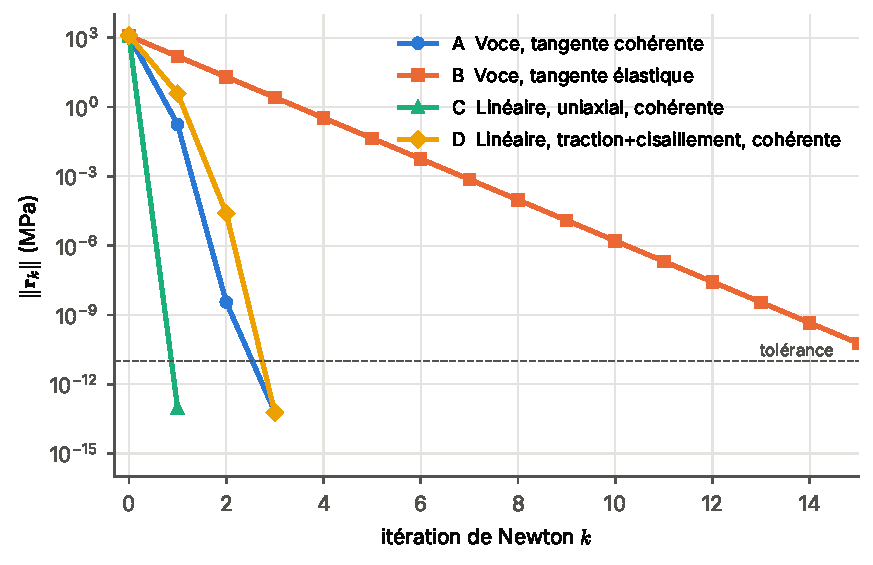
\includegraphics[width=0.78\linewidth]{newton_convergence}
\caption{Norme du résidu (MPa) au cours des itérations de Newton, pour un incrément $\varepsilon_{11}:0{,}1\,\%\to0{,}6\,\%$.}\label{fig:newton}
\end{figure}

\subsection{Résultats}

\begin{table}[h]
\centering
\begin{tabular}{llcc}
\toprule
Cas & Tangente & Itérations & Ordre empirique~\eqref{eq:ordre}\\
\midrule
A : Voce, uniaxial & cohérente & 3 & 2,01\\
B : Voce, uniaxial & élastique & 16 & 1,00 (taux 0,130)\\
C : linéaire, uniaxial & cohérente & 1 & ---\\
D : linéaire, traction + cisaillement & cohérente & 3 & 2,07\\
\bottomrule
\end{tabular}
\caption{Convergence du Newton au point matériel (tolérance $10^{-11}$~MPa).}\label{tab:newton}
\end{table}

\paragraph{Cas A et D : convergence quadratique.} Les résidus successifs du cas A valent $1{,}2\times10^{3}$, $1{,}8\times10^{-1}$, $3{,}6\times10^{-9}$ puis $6\times10^{-14}$. L'exposant double à chaque itération et l'ordre mesuré vaut 2,01. C'est la signature de la tangente cohérente.

\paragraph{Cas B : convergence linéaire.} Avec la tangente élastique, le résidu est multiplié par 0,130 à chaque itération, avec une régularité remarquable : l'ordre vaut 1,00 sur 15 itérations. Ce taux se \emph{prédit}. L'itération de Newton modifiée propage l'erreur par $\mathbf{M}=\mathbf{I}-\mathbf{K}_{e,ff}^{-1}\mathbf{K}_{t,ff}$. Le calcul des valeurs propres de $\mathbf{M}$ au point solution donne 0,1296 pour le mode symétrique $\delta\varepsilon_{22}=\delta\varepsilon_{33}$, et 0,797 pour les modes de cisaillement. Le résidu initial étant purement « latéral », seul le mode symétrique est excité, et on mesure 0,1296. Un chargement de cisaillement aurait convergé au taux 0,8, soit environ 110 itérations pour gagner 11 ordres de grandeur.

\paragraph{Cas C : le piège du sujet.} Avec un écrouissage linéaire en traction proportionnelle, Newton converge en \textbf{une seule} itération. On ne peut donc pas y observer de convergence quadratique. Ce n'est pas un bug : c'est une propriété du problème.

\begin{proposition}
Pour l'écrouissage isotrope (et cinématique) linéaire, en chargement uniaxial proportionnel ($\varepsilon_{22}=\varepsilon_{33}$, état initial de la même forme), la fonction $\varepsilon_{22}\mapsto\sigma_{22}$ calculée par le retour radial est affine par morceaux.
\end{proposition}
\begin{proof}
Toutes les déformations en jeu sont de la forme $a\,\I+b\,\mathbf{D}$ avec $\mathbf{D}=\mathrm{diag}(2,-1,-1)$, et $\epsp_n$, $\X_n$ sont proportionnels à $\mathbf{D}$. Donc $\bs\xi\tri=\beta\,\mathbf{D}$ avec $\beta$ affine en $\varepsilon_{22}$, et sa direction $\n=\pm\mathbf{D}/\|\mathbf{D}\|$ est \emph{constante} par morceaux (selon le signe de $\beta$). Alors $q\tri=\sqrt{3/2}\,\|\mathbf{D}\|\,|\beta|$ est affine par morceaux, $\Delta p=(q\tri-R(p_n))/(3\mu+h)$ l'est aussi, et $\sig_{n+1}=\sig\tri-2\mu\Delta p\N$ est affine par morceaux en $\varepsilon_{22}$. Newton résout exactement un problème affine en une itération, dès que l'itéré est dans le bon morceau (élastique ou plastique).
\end{proof}

La non-linéarité qui rend la tangente cohérente indispensable a deux sources : la courbure de $R(p)$ (cas A) et la \emph{rotation} de la direction d'écoulement $\n$ (cas D, où le rapport cisaillement/traction change au cours du pas). Dans un vrai calcul de structure, les deux sont presque toujours présentes. Pour \emph{démontrer} la convergence quadratique sur un point matériel, il faut donc choisir l'un de ces deux ingrédients.

\subsection{Chargement cyclique et hystérésis}

On impose $\varepsilon_{11}$ en triangle d'amplitude $\pm0{,}8\,\%$ pendant 3 cycles, avec contraintes latérales nulles, pour trois écrouissages (figure~\ref{fig:hyst}).

\begin{figure}[h]
\centering
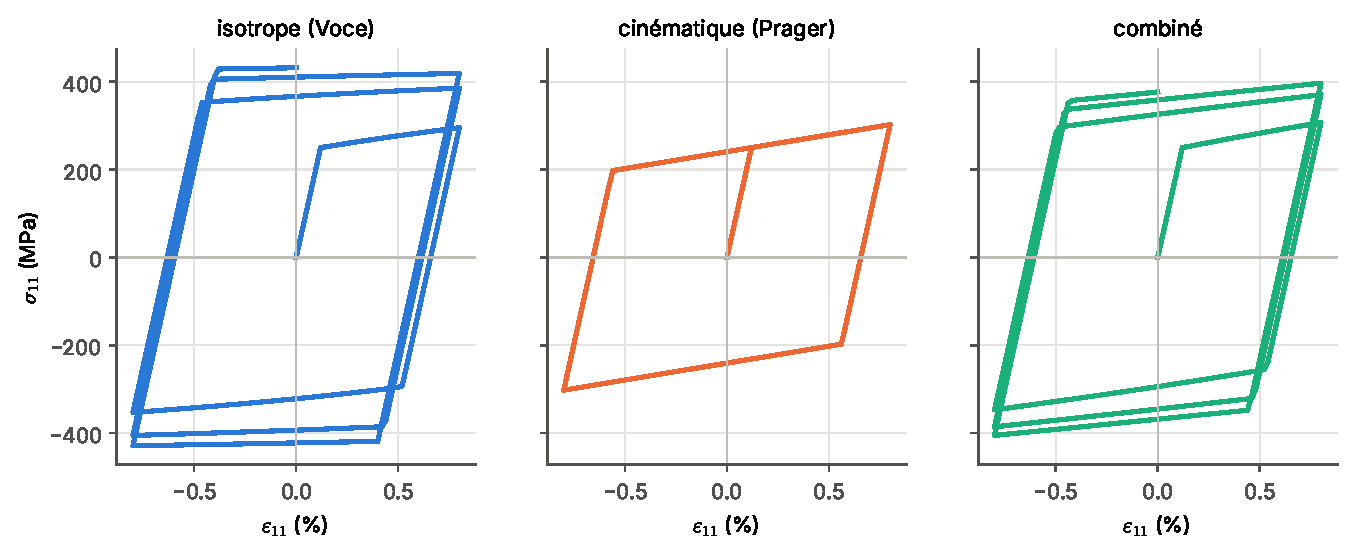
\includegraphics[width=\linewidth]{hysteresis}
\caption{Boucles contrainte--déformation en traction--compression cyclique (3 cycles, $\pm0{,}8\,\%$). Isotrope : $H=0{,}5$~GPa, $Q=150$~MPa, $b=50$. Cinématique : $C=8$~GPa. Combiné : $H=0{,}5$~GPa, $Q=100$~MPa, $b=50$, $C=4$~GPa.}\label{fig:hyst}
\end{figure}

\begin{itemize}
  \item \textbf{Isotrope.} Le domaine d'élasticité grossit à chaque passage plastique. Le pic de traction passe de 295~MPa au premier cycle à 419~MPa au troisième, et le pic de compression de $-353$ à $-429$~MPa. En inversion de charge, la plastification ne commence qu'à $-\sigma_{\text{pic}}$ : il n'y a \emph{pas} d'effet Bauschinger, ce qui est contraire à l'expérience sur les métaux.
  \item \textbf{Cinématique.} Le domaine garde sa taille ($2\sigma_y=500$~MPa) et se translate. Après une traction jusqu'à $+302{,}5$~MPa, la plastification inverse commence vers $302{,}5-500$, soit $-197{,}5$~MPa : c'est l'effet Bauschinger. La boucle est stabilisée dès le premier cycle et se superpose ensuite à elle-même.
  \item \textbf{Combiné.} Les deux mécanismes coexistent : on voit un effet Bauschinger et une boucle qui grossit en tendant vers une saturation, au rythme de $R(p)$ (pics de traction de 307 puis 371 et 397~MPa, de compression de $-347$ à $-406$~MPa). C'est le comportement qualitatif d'un acier, que les lois de type Chaboche affinent avec un écrouissage cinématique non linéaire.
\end{itemize}
Le Newton converge en au plus 3 itérations à chaque pas, y compris aux inversions de charge, où le pas passe du plastique à l'élastique.
